\chapter{Study of Literature}

\textbf{Author: } 

\section{Different Approaches to the Problem}
Localising a robot in an unknown surrounding can be achieved by a multitude of different sensors. To name a few stereo cameras, LIDAR systems, ultrasonic sensors and time-of-flight cameras all measure the distance to the objects located around the robot. This data can then be used to gather information about the current location of the robot or aid navigation.

\section{Stereo Camera}
The challenge of sensing distances to various objects has been solved using stereo vision cameras. Computer stereo vision systems use two horizontally displaced cameras to take two images which then are both processed together to gather the information on the depth of the images. This process can be rather complicated as the distortions of the images have to be undone, before the two images can be projected onto a common plane, a disparity map can be created by comparing the two images and a 3d point cloud can be generated from this comparison. In most robotics applications this point cloud is then filtered in search of some object, which distance was sought-after.

\subsection{Distortion}
One of the distortions that have to be undone before the images can be processed any further is called barrel distortion. It occurs when the lens used by the camera has a higher magnification at the centre of the image than at the sides. This distortion can be visualized as seen in Figure~\ref{pic:methodology_stereoCamera_distortion_barrelDistortion}.

\begin{figure}[h!]
	\centering
	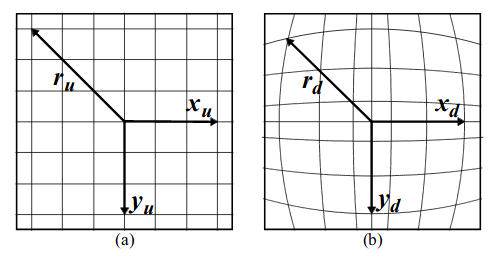
\includegraphics[width=4.5in]{img/methodology_stereoCamera_distortion_barrelDistortion.png}
	\caption{The left shows the original image composed of straight horizontal and vertical lines. On the right image the effect of the barrel distortion can be seen. The distortion causes the lines to curve toward the outside of the image, causing the lines to appear in a barrel like shape. [TODO: change image to own]}
	\label{pic:methodology_stereoCamera_distortion_barrelDistortion}
\end{figure}

Gribbon et.al. \footcite{Gribbon_Barrel_Distortion_Correction_Algorithm} propose equations, which calculate the pixel values in the undistorted image based on the pixel values in the distorted image.

In comparison to barrel distortion tangential distortion displaces points along the tangent of a circle placed at the centre of the image as seen in Figure~\ref{pic:methodology_stereoCamera_distortion_tangentialDistortion}.

\begin{figure}[h!]
	\centering
	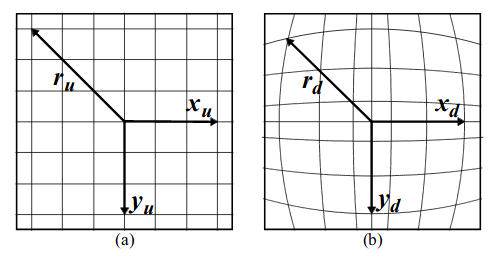
\includegraphics[width=2in]{img/methodology_stereoCamera_distortion_tangentialDistortion.png}
	\caption{A point $P$ is distorted along the tangent $t$ of a circle placed at the middle of the image $C$ with a radius $r$ to a point $P'$. Distortions of this form are called tangential distortions.}
	\label{pic:methodology_stereoCamera_distortion_tangentialDistortion}
\end{figure}

The radius of the circle in Figure~\ref{pic:methodology_stereoCamera_distortion_tangentialDistortion} is dependent on the point $P$. It can be calculated as the length between $P$ and $C$. The length of the vector $PP'$ is not uniform for all points and therefore depends on point $P$.

\subsection{Image Rectification}
Image Rectification projects multiple images taken from different points of view onto a common plane. 

\begin{figure}[h!]
	\centering
	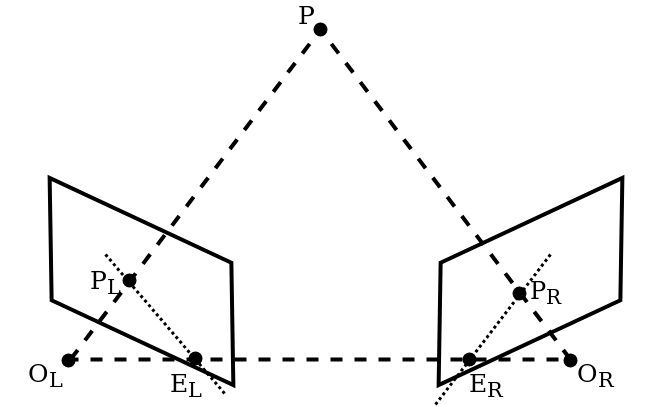
\includegraphics[width=4in]{img/methodology_stereoCamera_imageRectification.png}
	\caption{Two images containing some point $P$ are taken from the two points $O_L$ and $O_R$. Point $P$ is projected in the image planes as points $P_L$ and $P_R$. $E_L$ and $E_R$ depict the epipoles.}
	\label{pic:methodology_stereoCamera_imageRectification}
\end{figure}

Chan et. al. propose an image rectification algorithm \footcite{Chen_New_Image_Rectification_Algorithm}, which follows the following sequence of events:

\begin{enumerate}
	\item At least seven matching points visible on both images are found.
	\item The fundamental matrix (as well as the epipoles) are estimated.
	\item The common region is identified (using epipolar geometry constraints).
	\item The epipolar line is transferred and the Bresenham algorithm\footcite{Bresenham_Linear_Algorithm_For_Incremental_Digital_Display_Of_Circular_Arcs} is used to extract pixel values.
	\item The rectified image is resampled.
\end{enumerate}

\subsection{Disparity Map}
A disparity map represents the depth of an image. It can be calculated by comparing the position of pixels in two images made for example by a stereo camera. Objects, that are closer, have a larger difference in their relative position on the two image, than objects that are farther away.

One approach, which focuses not only on the quality of the disparity, but also on the time needed to compute the result, is described in the work of Mühlmann et.al\footcite{Muehlmann_Calculating_Dense_Disparity_Maps_from_Color_Stereo_Images}.

\subsection{3d point cloud}
To generate a 3d point cloud out of the disparity map a two dimensional image has to be converted into a three dimensional space. This is done by extracting the information about the depth for each pixel from the disparity map. In our use case the resulting 3d point cloud then has to be filtered in search of the object, which distance to was sought after.

\section{LIDAR}

\section{Structure from Motion}

\section{Feature Tracking}

\section{Depth perception}
[TODO: humans, two eyes - gleich wie bei unserem Aufbau]

\subsection{Depth sensation}
[TODO: Pigeons, deer, children (visual cliff)]


\filbreak